\documentclass[11pt]{beamer}
\usetheme{Boadilla}
\usepackage[utf8]{inputenc}
\usepackage{amsmath}
\usepackage{amsfonts}
\usepackage{amssymb}
\usepackage{graphicx}
\usepackage{tabularx}
\usepackage{tikz}
\usetikzlibrary{arrows,shapes.geometric,positioning}
\usepackage{pifont}% http://ctan.org/pkg/pifont
\newcommand{\xmark}{\ding{55}}%
% Define block styles
\tikzstyle{block} = [rectangle, draw, fill=blue!20, 
    text width=9.5em, text centered, rounded corners, minimum height=4em]
\tikzstyle{line} = [draw, -latex]

\graphicspath{{fig/}}

\author[Weiyao Ke]{Weiyao Ke, J Scott Moreland, Jonah E Bernhard, and Steffen A Bass}
\title[3D Initial Condition]{Constraining 3D Hydrodynamic Initial Condition for Relativistic Heavy-ion Collisions from Multiplicity Observables of pA and AA @LHC}

%\setbeamercovered{transparent}
%\setbeamertemplate{navigation symbols}{}
%\logo{qcdlogo.pdf}
\institute{Duke University}
\date{\today}
%\subject{}
\newcommand{\TRENTo}{T\raisebox{-0.2em}{R}ENTo~}
\begin{document}

\begin{frame}
\titlepage
\begin{center}
\small arXiv:1610.08490
\end{center}
\end{frame}

\section{Initial condition for 3+1D simulation}
\begin{frame}{Initial condition for 3+1D simulation}
\begin{itemize}
\item Relativistic viscous hydrodynamics is one of the key tools to study heavy ion collisions.
\item Hydrodynamics initial condition (complicated): energy/entropy density, fluid velocity, stress tensor...
\item Initial condition uncertainties propagate to the extraction of QGP properties.
\item Continuous progress in first principal calculation of both 2D (beam direction invariant) and 3D initial condition, but very hard!
\end{itemize}
\begin{center}
\color{red} What can we learn about 3D initial condition from data?
\end{center}
\end{frame}

\begin{frame}{Longitudinal fluctuations and asymmetries}
\begin{itemize}
\item For midrapidity observables, one usually neglects evolution in the beam direction.
\item For rapidity dependent observables, includes longitudinal fluctuations.
\begin{center}
\includegraphics[width=0.6\textwidth]{nuclei_demo.pdf}
%\includegraphics[width=0.3\textwidth]{pPb.pdf} 
\end{center}
\item For small collision system: even stronger asymmetry.
\end{itemize}
\end{frame}

\section{Parametric longitudinal information}
\begin{frame}{Midrapidity: phenomenological model \TRENTo \tiny PRC 92, 011901(2015)}
\begin{itemize}
\item Nucleons are sampled from Woods-Saxon distribution.
\item Participants: nucleons participant at least one binary collisions.
\item Nuclear thickness function, ${\color{blue} T_{A, B}(x_\perp)} = \int dz \rho_{A, B}^{}(z, x_\perp)$.
\end{itemize}

\begin{columns}
\begin{column}{0.65\textwidth}
\begin{itemize}
\item \TRENTo: mappings from ${\color{blue} T_A(x_\perp), T_B(x_\perp)}$ to midrapidity {\color{red} entropy production},
\begin{eqnarray}
\nonumber
{\color{red} s_0(x_\perp, \eta=0)} \propto \left(\frac{{\color{blue} T_A}^p + {\color{blue} T_B}^p}{2}\right)^{1/p}.
\end{eqnarray}
$p$: a tunable parameter. \TRENTo mimics and interpolates between different initial condition models.
\end{itemize}
\end{column}
\begin{column}{0.35\textwidth}
\includegraphics[width=\textwidth]{overlap_3.pdf}\\
\includegraphics[width=\textwidth]{traincar-crop.pdf}\\
\begin{center}
\tiny by J S Moreland
\end{center}
\end{column}
\end{columns}
\end{frame}

\begin{frame}{Extending \TRENTo to finite rapidity}
\begin{itemize}
\item The formula,
\begin{eqnarray}\nonumber 
\frac{dS}{dx_\perp^2d y} \propto  s_0(\vec{x}_\perp) {\color{red}f(y, x_\perp)}.
\end{eqnarray} 
\item $s_0$: original \TRENTo prediction.
\item {\color{red} $f(y, x_\perp)$}: rapidity profile with three degrees of freedom,\\
mean ($\mu$), std ($\sigma$), skewness ($\gamma$), (the first three moments).
\begin{eqnarray}\nonumber 
f(y) \propto \mathcal{F}^{-1}\exp\left\{ik\mu(x_\perp) -\frac{1}{2}[\sigma(x_\perp) k]^2 - \frac{i}{6}\gamma(x_\perp)[\sigma(x_\perp) k]^3 + ...\right\}
\end{eqnarray}
\item $\mu$, $\sigma$, $\gamma$ parametrized in nuclear thickness functions.
\end{itemize}
\begin{center}
\begin{tabularx}{0.95\textwidth}{p{2.3cm}p{1.2cm}p{8.2cm}}
\hline
mean($\mu$) & std($\sigma$) &$\left.\right.${\color{red!70}absolute} or {\color{blue!70}relative}-skewness($\gamma$) \\
\hline
\noalign{\smallskip}
$\frac{\mu_0}{2} \log\frac{T_A(x_\perp)}{T_B(x_\perp)}$ & $\sigma_0$ & $\left.\right.${\color{red!70}$\gamma_0(T_A(x_\perp)-T_B(x_\perp))$} 
or 
{\color{blue!70}$\gamma_0\frac{T_A(x_\perp)-T_B(x_\perp)}{T_A(x_\perp)+T_B(x_\perp)}$} \\
\noalign{\smallskip}
\hline
\end{tabularx}
\end{center}
\end{frame}

\section{Model to data comparison}
\begin{frame}{Model-to-data comparison}
Model: T\raisebox{-0.2em}{R}ENTo-3D, 3+1D Hydro {\tiny (CPC 185 (2014), 3016)}, Ultra relativistic Quantum Molecular Dynamics (UrQMD, {\tiny Prog.Part.Nucl.Phys.41:255-369,1998})
\begin{itemize}
\item Summary of parameters:\\
"Transverse": normalizations, nucleon width, fluctuation, $p$.\\
"Longitudinal": $\mu_0,\sigma_0, \gamma_0$, Jacobian
\end{itemize}
Data: 
\begin{itemize}
\item Charged particle $\eta$-distribution (ALICE Pb+Pb 2.76TeV, ATLAS $p$+Pb 5.02 TeV), reflects centrality/$\eta$ dependent entropy production.
\item Two-particle $\eta$-correlation (ATLAS Pb+Pb 2.76 TeV), 
sensitive to amount of longitudinal fluctuation.
\end{itemize}
Assuming viscous effects on the total multiplicity are mild, use ideal hydro as a first step.
\end{frame}

\begin{frame}{Bayesian model-to-data comparison}
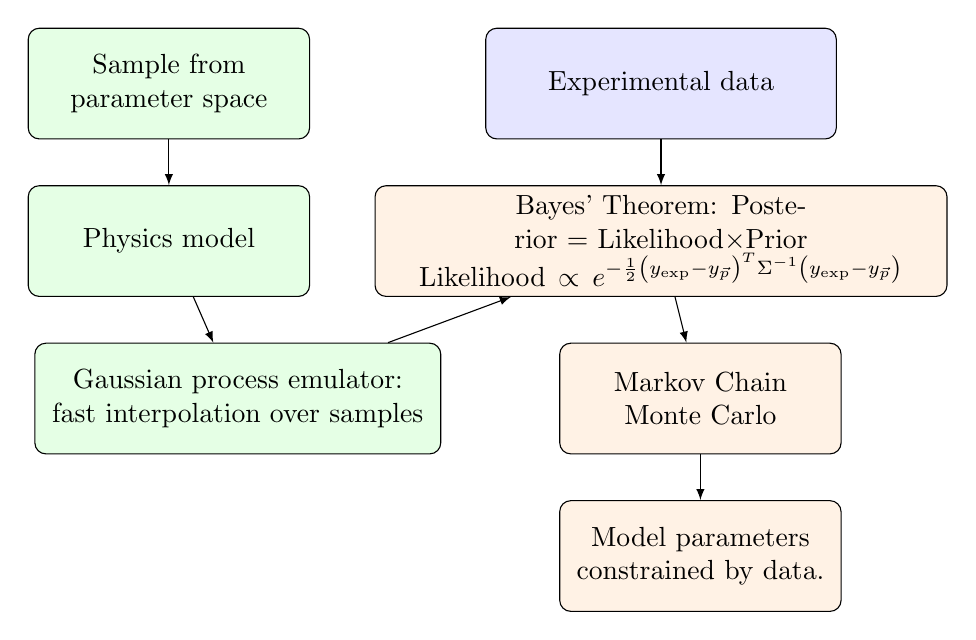
\begin{tikzpicture}[align=center,node distance=4cm]
    % Place nodes
    \node [block, fill=green!10] (param) {Sample from\\ parameter space};
    \node [block, fill=green!10, below of=param, yshift=2cm] (model) {Physics model};
    \node [block, text width=12em, fill=blue!10, right of=param, xshift=2.25cm] (exp) {Experimental data};
    \node [block, text width=14em, fill=green!10, below of=model, xshift=0.875cm, yshift=2cm] (GP) {Gaussian process emulator: fast interpolation over samples};
    \node [block, text width=20em, fill=orange!10, right of=model, xshift=2.25cm] (Bayes) {
    Bayes' Theorem: Posterior = Likelihood$\times$Prior\\ 
    $\textrm{Likelihood} \propto e^{-\frac{1}{2} \left(y_{\textrm{exp}} - y_{\vec{p}} \right)^T \Sigma^{-1} \left(y_{\textrm{exp}} - y_{\vec{p}} \right)}$
    };
	\node [block, fill=orange!10, below of=Bayes, xshift=0.5cm, yshift=2cm] (MCMC) {Markov Chain Monte Carlo};
	\node [block, fill=orange!10, below of=MCMC, yshift=2cm] (posterior) {Model parameters constrained by data.};
    % Draw edges
    \path [line] (param)-- (model);
    \path [line] (model) -- (GP);
    \path [line] (GP) -- (Bayes);
    \path [line] (exp) -- (Bayes);
   	\path [line] (Bayes) -- (MCMC);
   	\path [line] (MCMC) -- (posterior);

\end{tikzpicture}
\end{frame}

\section{Constraint initial condition and predictions}
\begin{frame}{After fitting to data: posterior observables}
\begin{itemize}
\item Nicely fit the centrality $\&$ pseudorapidity dependence of $dN_{ch}/d\eta$.
\item $\left\langle a_1^2\right\rangle^{1/2}$: initial condition + hydro approach for two particle $\eta$-correlation breaks down at large centrality.
\end{itemize}
\includegraphics[width=\textwidth]{post_obs.pdf}\\
\tiny  	PLB 726 (2013) 610-622, PLB 754 (2016) 373-385, EPJ C (2016) 76:199, Nucl. Part. Phys. Proc. 276–278, 121 (2016).
\end{frame}

\begin{frame}{Posterior $dS/d\eta$ for various value of $T_A$ and $T_B$}
\begin{itemize}
\item 3D entropy production is reverse engineered from multiplicity data.
\begin{columns}
\begin{column}{0.6\textwidth}
\includegraphics[width=\textwidth]{post_dsdy.pdf}
\end{column}
\begin{column}{0.4\textwidth}
\begin{itemize}
\item Figure shows $ds/d\eta$ varying $T_A$, $T_B$.
\item Imbalance \& fluctuations of $T_A$, $T_B$ lead to asymmetric local entropy production.
\item What's still missing: fluctuation from early time dynamics.
\end{itemize}
\end{column}
\end{columns}
\end{itemize}
\end{frame}

\begin{frame}{Calculation of azimuthal correlation observables}
\begin{itemize}
\item We select parameters from posterior. Use viscous hydro ($\eta/s = 0.25$) + UrQMD to calculate $v_n\{2\}$, $v_2\{4\}$, and event-plane decorrelations.
\end{itemize}
\includegraphics[width=0.59\textwidth]{vn_eta.pdf}\hfill
\includegraphics[width=0.325\textwidth]{evt_pln_decorr_near.pdf}\\
\tiny PLB 762 (2016) 376-388, PRC 92 (2015) 034911
\end{frame}

\begin{frame}{Summary}
\begin{itemize}
\item \TRENTo initial condition is extended to include rapidity dependence.
\item The multiplicity data over-constrains the model parameters.
\item \colorbox{red!20}{Initial 3D entropy production reverse engineered
 from experiments.}
\item \colorbox{blue!20}{Provide guidance for first principal calculation.}
\item \colorbox{blue!20}{Could benefit small collision system simulations.}
\end{itemize}
\end{frame}

\begin{frame}[noframenumbering]{Back up: full nine-parameter posterior}
\begin{center}
\includegraphics[width=0.7\textwidth]{posterior.pdf}
\end{center}
\end{frame}

\begin{frame}[noframenumbering]{Back up: Flow at midrapidity}
\begin{center}
\includegraphics[width=0.8\textwidth]{vn_cen.pdf}
\end{center}
\end{frame}

\begin{frame}[noframenumbering]{Back up: event-plane decorrelation}
\begin{center}
\includegraphics[width=0.45\textwidth]{evt_pln_decorr_near.pdf}
\quad\quad
\includegraphics[width=0.45\textwidth]{evt_pln_decorr_far.pdf}
\end{center}
\end{frame}

\begin{frame}[noframenumbering]{Back up: calculation of symmetric cumulants}
\begin{center}
\includegraphics[width=\textwidth]{smn.pdf}
\end{center}
\end{frame}

\begin{frame}[noframenumbering]{Back up: Inverse the cumulant generating function}
To ensure the function inversed from cumulant generating function has good properties, 
\begin{eqnarray}
&-3.3\sigma < y < 3.3\sigma, \\
&\gamma \rightarrow \gamma\exp\left(-\frac{1}{2}\sigma^2k^2\right).
\end{eqnarray}
\begin{center}
\includegraphics[width=0.7\textwidth]{regulate.pdf}
\end{center}
\end{frame}

\begin{frame}[noframenumbering]{Back up: Two particle $\eta$-correlation}
Expand event-wise $dN/d\eta$ in Legendre Polynomials (within $|\eta|<Y$). 
\begin{eqnarray}
\nonumber
\frac{dN}{d\eta} = \left\langle \frac{dN}{d\eta} \right\rangle \left(a_0 + a_1 P_1\left(\frac{\eta}{Y}\right) + a_2 P_2\left(\frac{\eta}{Y}\right) + ...\right)
\end{eqnarray}
The correlations between the expansion coefficients are related to the two particle $\eta$-correlation function,
\begin{eqnarray}
\nonumber
C(\eta_1,\eta_2) &=& \frac{\left\langle dN(\eta_1)dN(\eta_2)\right\rangle}{\left\langle dN(\eta_1)\right\rangle\left\langle dN(\eta_2)\right\rangle}-1\\
\nonumber
\left\langle a_n a_m\right\rangle &=& \frac{(2n+1)(2m+1)}{4} \int \frac{d\eta_1}{Y}\frac{d\eta_2}{Y} C(\eta_1,\eta_2)T_{mn}(\eta_1,\eta_2)\\
T_{mn}(1,2) &=& \frac{P_m(1)P_n(2)+P_m(2)P_n(1)}{2}
\end{eqnarray}
\end{frame}


\end{document}
